\documentclass[10pt]{beamer}
\usetheme{Singapore}
\usecolortheme{default}
\usecolortheme{orchid}
\useoutertheme{infolines}
\useinnertheme[shadow=true]{rounded}

\newcommand\tinyfont{\fontsize{4pt}{7.2}\selectfont}
\newcommand\smallfont{\fontsize{8pt}{7.2}\selectfont}
\newcommand\regfont{\fontsize{10pt}{7.2}\selectfont}

\usepackage{multimedia}
\usepackage{pdfpages}

\begin{document}

\title{Using the Yale HPC Clusters}`
\titlegraphic{
\includegraphics[height=2.0cm]{logo.png}}
\logo{
\includegraphics[height=0.5cm]{logo.png}}
\author{{Robert Bjornson}}
\institute[Yale]{
  Yale Center for Research Computing \\
  Yale University
}
\date{Jan 2018}

%----------- titlepage ----------------------------------------------%
\begin{frame}[plain]
  \titlepage
\end{frame}

%----------- slide ----------------------------------------------%
\begin{frame}[fragile]
\frametitle{Getting the Workshop Slides and Demos}
\begin{itemize}
\item https://github.com/ycrc/Intro-Bootcamp
\item clone (if you know how)
\item or download zip and unpack
\item slides are hpc.pdf
\end{itemize}
\end{frame}

%----------- slide --------------------------------------------------%
\begin{frame}[fragile]
\frametitle{What is the Yale Center for Research Computing?}

\begin{itemize}
\item Independent center under the Provost's office
\item Created to support your research computing needs
\item Focus is on high performance computing and storage
\item \textasciitilde 15 staff, including applications specialists and system engineers
\item Available to consult with and educate users
\item Manage compute clusters and support users
\item Located at 160 St. Ronan st, at the corner of Edwards and St. Ronan
\item http://research.computing.yale.edu
\end{itemize}

\end{frame}

%----------- slide --------------------------------------------------%
\begin{frame}
\frametitle{What is a cluster?}

A \textbf{cluster} usually consists of a hundred to a thousand rack mounted
computers, called \textbf{nodes}.  It has one or two \textbf{login nodes}
that are externally accessible, but most of the nodes are
compute nodes and are only accessed from a login node via a
\textbf{batch queueing system} (Slurm).

\vskip10pt
The CPU used in clusters may be similar to the CPU in your
desktop computer, but in other respects they are rather different.

\begin{itemize}
\item Linux operating system
\item Command line oriented 
\item Many cores (cpus) per node
\item No monitors, no CD/DVD drives, no audio or video cards
\item Lots of RAM
\item Very large distributed file system(s)
\item Connected internally by a fast network
\end{itemize}
\end{frame}

%----------- slide ----------------------------------------------%
\begin{frame}[fragile]
\frametitle{Compute Cluster Schematic}

\begin{center} 
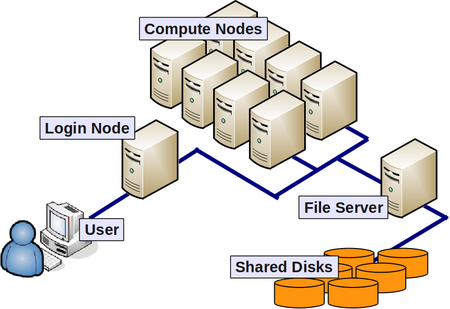
\includegraphics[height=5cm]{cluster.png} 
\end{center}
\end{frame}

%----------- slide ----------------------------------------------%
\begin{frame}[fragile]
\frametitle{Yale Compute Cluster}

\begin{center}
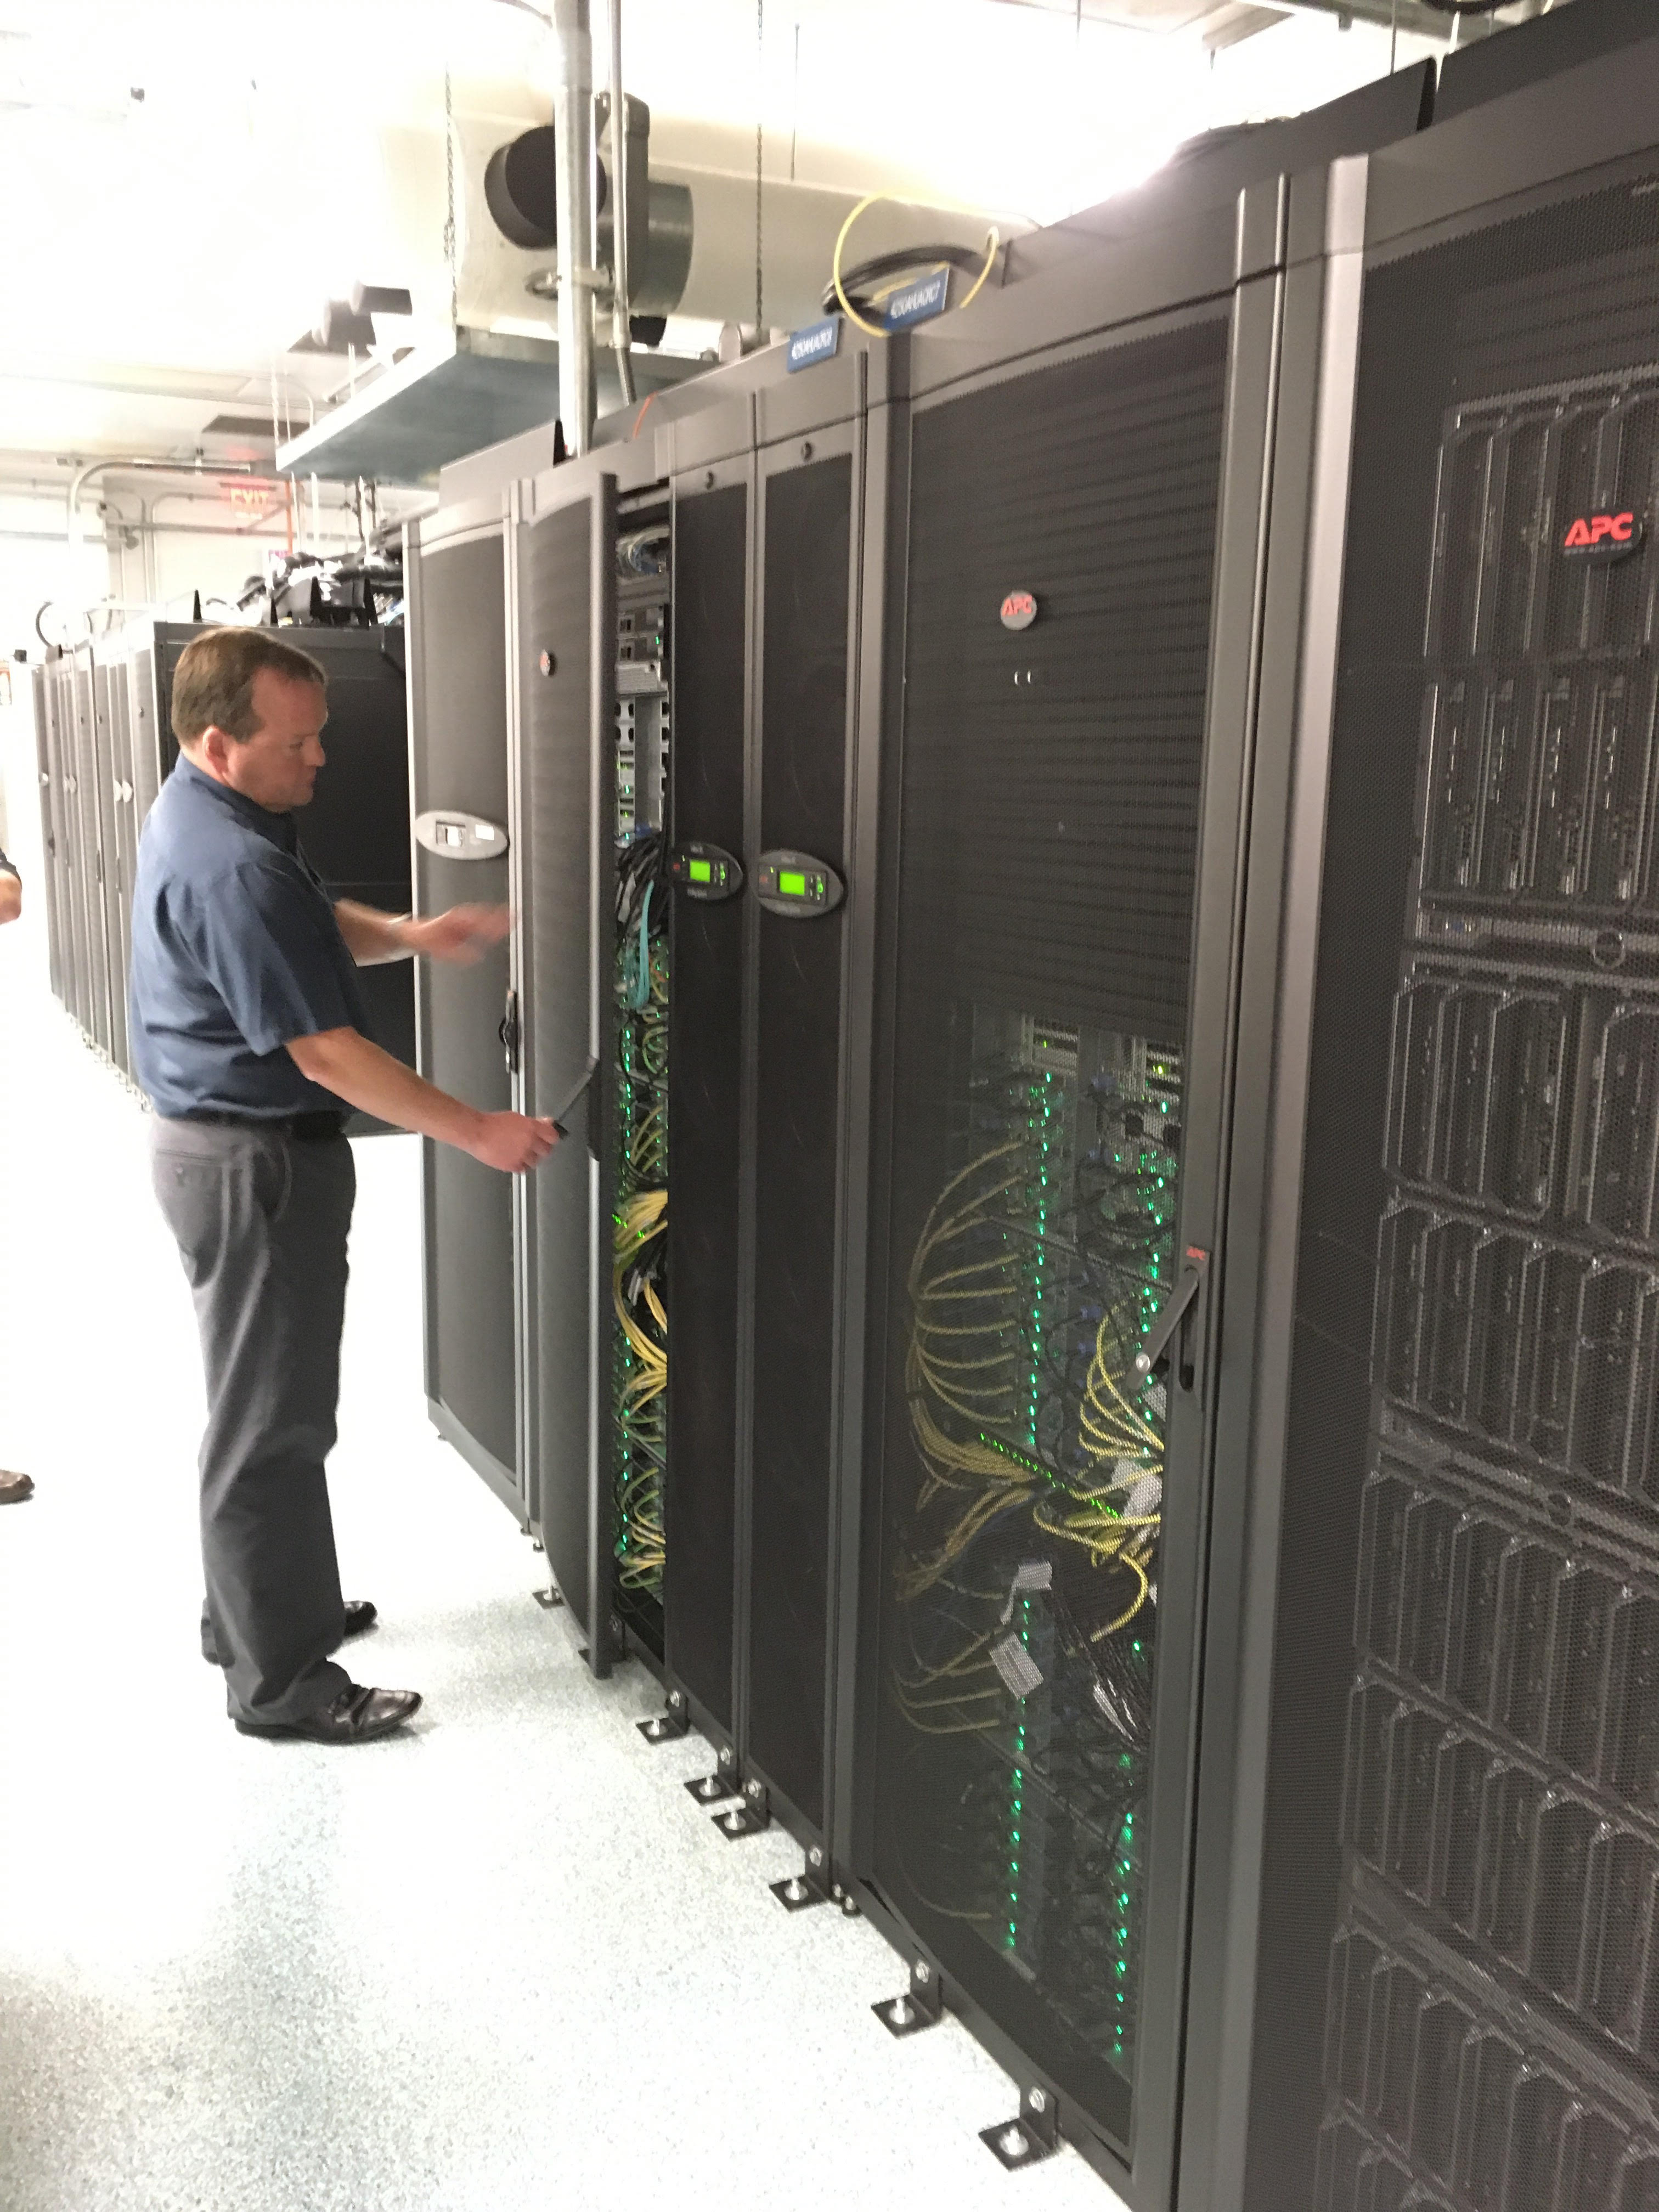
\includegraphics[height=7cm]{yalecluster.jpg}
\end{center}

\end{frame}

%----------- slide --------------------------------------------------%
\begin{frame}
\frametitle{Why use a cluster?}
Clusters are very powerful and useful, but it may take some
time to get used to them.
Here are some reasons to go to that effort:

\begin{itemize}
\item Don't want to tie up your own machine for many hours or days
\item Have many long running jobs to run
\item Want to run in parallel to get results quicker
\item Need more disk space
\item Need more memory
\item Want to use software installed on the cluster
\item Want to access data stored on the cluster
\item Want to use GPUs
\end{itemize}
\end{frame}

%----------- slide --------------------------------------------------%
\begin{frame}
\frametitle{Limitations of clusters}
Clusters are not the answer to all large scale computing problems.
Some of the limitations of clusters are:

\begin{itemize}
\item Cannot run Windows or Mac programs
\item Not for persistent services (DBs or web servers)
\item Not ideal for interactive, graphical tasks
\item Jobs that run for weeks can be a problem (unless checkpointed)
\end{itemize}
\end{frame}

%----------- slide --------------------------------------------------%
\begin{frame}[fragile]
\frametitle{Summary of Yale Clusters (Jan 2018)}
\smallfont
\begin{tabular}{|c|c|c|c|c|c|}
\hline
& \textbf{Omega-next} & \textbf{Grace}& \textbf{Farnam} & \textbf{Ruddle} & \textbf{Milgram} \\
\hline
\textbf{Role} & FAS & FAS & LS/Med & YCGA & Psych \\
\hline
\textbf{~Total nodes} & 1028* & 216 & 320+ & 156+ & 60 \\
\hline
\textbf{~Total cores} & 8500* & 4700 & 5300 & 3000 & ~1500 \\
\hline
\textbf{Cores/node} & 8 & 20 & 8-20 & 20 & 20-28 \\
\hline
\textbf{GB/node} & 128 & 128-256 & \multicolumn{2}{|c|}{128-1500} & 128-256 \\
\hline
\textbf{Network} & QDR IB & FDR IB & \multicolumn{3}{|c|}{10 Gb EN}   \\
\hline
\textbf{File system} & Lustre+GPFS & GPFS & GPFS & NAS + GPFS & GPFS \\
\hline
\textbf{Batch queueing} & \multicolumn{5}{|c|}{Slurm}  \\
\hline
\textbf{GPU nodes} & No & Several & Few & No & No \\
\hline
\textbf{Duo MFA?} & No & No & No & Yes & No \\
\hline
\end{tabular}
\regfont
\vskip10pt
* Transition from omega to omega-next ongoing
\vskip 10pt
Details on each cluster here:
\url{http://research.computing.yale.edu/hpc-clusters}

\end{frame}

%----------- slide --------------------------------------------------%
\begin{frame}[fragile]
\frametitle{Setting up a account}

Accounts are free of charge to Yale researchers.
\vskip10pt

Request an account at: \url{http://research.computing.yale.edu/account-request}.

\vskip10pt
After your account has been approved and created, you will receive
an email describing how to access your account.  This may involve setting up ssh keys or 
using a secure login application.  Details vary by cluster.

\vskip10pt
If you need help setting up or using ssh, send an email to: \url{hpc@yale.edu}.
\end{frame}

%----------- slide --------------------------------------------------%
\begin{frame}[fragile]
\frametitle{Ssh to a login node}
To access any of the clusters, you must use \textbf{ssh}.
From a Mac or Linux machine, you simply use the \textbf{ssh} command:

\begin{verbatim}
laptop$ ssh netid@omega-next.hpc.yale.edu
laptop$ ssh netid@grace.hpc.yale.edu
laptop$ ssh netid@farnam.hpc.yale.edu
laptop$ ssh netid@ruddle.hpc.yale.edu
\end{verbatim}

From a Windows machine we recommend using putty: \url{http://www.putty.org}.

\vskip10pt
For more information on using PuTTY see:
\url{http://research.computing.yale.edu/hpc-support/user-guide/secure-shell-for-microsoft-windows}
\end{frame}

%----------- slide --------------------------------------------------%
\begin{frame}[fragile]
\frametitle{Understanding ssh key pairs}
\begin{itemize}
\item We use key pairs instead of passwords to log into clusters
\item Keys are generated as pair:
\begin{itemize}
\item ssh-keygen: public (id\_rsa.pub) and private (id\_rsa)
\item putty/winscp: public (name.pub) and private (name.ppk)
\end{itemize}
\item You should always use a pass phrase to protect private key!
\item You can freely give the public key to anyone
\item You can generate a new pair for each of your computers, or reuse the same pair.
\item NEVER give the private key to anyone!
\end{itemize}
\end{frame}

%----------- slide --------------------------------------------------%
\begin{frame}[fragile]

\frametitle{Outline of setting up keys}
\begin{enumerate}
\item Generate key pair using ssh-keygen (linux/mac) or puttygen (windows)
\item Locate the public and private key files you generated
\item Use our tool to upload the public key (link on page shown below)
\item Wait 15 minutes for key to propagate
\item Connect using private key
\end{enumerate}

This can be tricky the first time.  See http://research.computing.yale.edu/support/hpc/user-guide
for the exact steps or contact us if you have problems.

\end{frame}

%----------- slide --------------------------------------------------%
\begin{frame}[fragile]
\frametitle{Sshing to Ruddle}

\begin{itemize}
\item Ruddle has an additional level of ssh security, using Multi Factor Authentication (MFA)
\item We use Duo, the same MFA as other secure Yale sites
\end{itemize}

Example:
\begin{verbatim}
bjornson@debian:~$ ssh rdb9@ruddle.hpc.yale.edu
Enter passphrase for key '/home/bjornson/.ssh/id_rsa': 
Duo two-factor login for rdb9

Enter a passcode or select one of the following options:

 1. Duo Push to XXX-XXX-9022
 2. Phone call to XXX-XXX-9022
 3. SMS passcodes to XXX-XXX-9022

Passcode or option (1-3): 1
Success. Logging you in...
\end{verbatim}  
\end{frame}

%----------- slide --------------------------------------------------%
\begin{frame}[fragile]
\frametitle{More about MFA}

\begin{itemize}
\item Don't have a smartphone? Get a hardware device from the ITS Helpdesk
\item Register another phone: e.g your home or office phone, as a backup
\item See http://research.computing.yale.edu/support/hpc/user-guide/mfa
\end{itemize}


\end{frame}
%----------- slide --------------------------------------------------%
\begin{frame}[fragile]
\frametitle{Running jobs on a cluster}

Two ways to run jobs on a cluster:

Interactive:
\begin{itemize}
\item you request an allocation
\item system grants you one or more nodes
\item you are logged onto one of those nodes
\item you run commands
\item you exit and system automatically releases nodes
\end{itemize}

Batch:
\begin{itemize}
\item you write a job script containing commands
\item you submit the script
\item system grants you one or more nodes
\item your script is automatically run on one of the nodes
\item your script terminates and system releases nodes
\item system sends a notification via email
\end{itemize}

\end{frame}

%----------- slide --------------------------------------------------%
\begin{frame}[fragile]
\frametitle{Interactive vs. Batch}

Interactive jobs:
\begin{itemize}
\item like a remote session
\item require an active connection
\item for development, debugging, or 
interactive environments like R and Matlab 
\end{itemize}
\vskip10pt

Batch jobs:
\begin{itemize}
\item non-interactive  
\item can run many jobs simultaneously
\item your best choice for production computing
\end{itemize}
\end{frame}

%----------- slide --------------------------------------------------%                                                                                                                              
\begin{frame}[fragile]
\frametitle{General overview of Slurm}

Slurm manages all the details of cluster operation:
\begin{itemize}
\item Interactive node allocation
\item Batch job submission
\item Specifying and reserving the resources you need for your job
\item Listing running and pending jobs
\item Cancelling jobs
\item Grouping node resources into partitions
\item Prioritizing and scheduling jobs
\end{itemize}

For information specific to each cluster:
http://research.computing.yale.edu/support/hpc/clusters

\end{frame}

%----------- slide --------------------------------------------------%
\begin{frame}[fragile]
\frametitle{Interactive allocations}

\begin{verbatim}

srun -p interactive --pty bash

\end{verbatim}

You'll be logged into a compute node and can run your commands. 
\vspace{0.1in}
To exit, type exit or ctrl-d

\end{frame}

%----------- slide --------------------------------------------------%
\begin{frame}[fragile]
\frametitle{Slurm: Example of an interactive job}
\begin{verbatim}
farnam-0:~ $ srun --pty -p interactive --mem=8g bash
c01n01$ module load Bowtie2
c01n01$ bowtie2 -1 data/sample_R1.fastq -2 data/sample_R2.fastq \
    -x hg19/genome > output.sam
c01n01$ exit
farnam-0:~ $
\end{verbatim}
\end{frame}

%----------- slide --------------------------------------------------%
\begin{frame}[fragile]
\frametitle{Batch jobs}
\begin{itemize}
\item create a script wrapping your job
\item declares resources required
\item contains the command(s) to run
\end{itemize}

\end{frame}

%----------- slide --------------------------------------------------%
\begin{frame}[fragile]
\frametitle{Slurm: Example of a batch script}

\begin{block}{}
\begin{verbatim}

#!/bin/bash
#SBATCH --mail-type=ALL
#SBATCH --mail-user=robert.bjornson@yale.edu
#SBATCH -t 3:00 # 3 minutes
#SBATCH --mem=10g

module load R

Rscript myscript.R
\end{verbatim}
\end{block}{}
\end{frame}

%----------- slide --------------------------------------------------%
\begin{frame}[fragile]
\frametitle{Slurm: Example of a batch job}
\smallfont
\begin{verbatim}
$ sbatch batch.sh
Submitted batch job 42
$ squeue -j 42
JOBID PARTITION     NAME     USER ST       TIME  NODES NODELIST(REASON)
   42   general   batch     rdb9  R       0:03      1 c13n10
\end{verbatim}
\vskip14pt
\regfont
The script runs in the current directory.  
Output goes to slurm-\textit{jobid}.out by default, or use -o
\end{frame}


%----------- advanced slides ----------------------------------------%

%----------- slide --------------------------------------------------%
\begin{frame}[fragile]
\frametitle{Copy scripts and data to the cluster}
\begin{itemize}
\item On Linux and Mac, use scp and rsync
to copy scripts and data files from between local computer and cluster.

\begin{verbatim}
laptop$ scp -r ~/workdir netid@omega.hpc.yale.edu:
laptop$ rsync -av -e 'ssh -i ~/.ssh/id_rsa' ~/workdir \
        netid@grace.hpc.yale.edu:
\end{verbatim}

\item Cyberduck is a good graphical tool for Mac or Windows.  \url{https://cyberduck.io}

\item For Windows, WinSCP is available from the Yale Software
Library: \url{http://software.yale.edu}.

\item Graphical copy tools usually need configuration when used with Duo (Ruddle).  See:
http://research.computing.yale.edu/support/hpc/user-guide/transfer-files-or-cluster
\end{itemize}

\end{frame}

%----------- slide --------------------------------------------------%
\begin{frame}[fragile]
\frametitle{Summary of Slurm commands}
\begin{tabular}{|l|l|}
\hline
\textbf{Description} & \textbf{Command} \\
\hline
Submit a batch job & sbatch [\textit{opts}] \textit{SCRIPT} \\
\hline
Submit an interactive job & srun -p interactive -{}-pty [\textit{opts}] bash  \\
\hline
Status of a job & squeue -j \textit{JOBID} \\
\hline
Status of a user's jobs & squeue -u \textit{NETID} \\
\hline
Cancel a job & scancel \textit{JOBID} \\
\hline
Get job info for partition & squeue -p \textit{PART} \\
\hline
Get node info for partition & sinfo -p {PART} \\
\hline
Get individual node info & sinfo -N -n \textit{NODE} \\
\hline
Get job info & sacct -j \textit{JOBID} -l \\
\hline
\end{tabular}

\vspace{0.1in}
Useful formatting:
\smallfont
\begin{verbatim}
export SACCT_FORMAT="JobID%-20,JobName,User,Partition,NodeList,Elapsed,\
  State,ExitCode,MaxRSS, AllocTRES%32"

export SQUEUE_FORMAT="%.16i %.12P %.12j %.8u %.2t %.12M %.12l %20R %.6D \
  %.6C %.10m %8b %8f"
\end{verbatim}

\end{frame}

%----------- slide --------------------------------------------------%
\begin{frame}[fragile]
\frametitle{Summary of Slurm sbatch/srun options}
\begin{tabular}{|l|l|}
\hline
\textbf{Description} & \textbf{Option} \\
\hline
Partition & -p \textit{PART} \\
\hline
Process count & -c \textit{CPUS} \\
\hline
Node count & -N \textit{NODES} \\
\hline
Task count & -n \textit{TASKS} \\
\hline
Wall clock limit & -t \textit{HH}:\textit{MM} or \textit{DD}-\textit{HH}\\
\hline
Memory limit & -{}-mem 4g or -{}-mem-per-cpu 4g)\\
\hline
Interactive job & srun -{}-pty bash \\
\hline
Job name & -J \textit{NAME} \\
\hline
\end{tabular}

\vskip10pt
Examples:
\smallfont
\begin{verbatim}
farnam1$ srun --pty -p general --mem-per-cpu 32g -t 24:00 bash 
farnam1$ sbatch -p general --mem 8g -c 20 -t 3- job.sh   
\end{verbatim}
\end{frame}

%----------- slide --------------------------------------------------%
\begin{frame}[fragile]
\frametitle{Partitions}
\begin{itemize}
\item Compute nodes are grouped into partitions
\item Each cluster has its own set of partitions, see page
\item Jobs are submitted to a specific partition
\item Each partition has rules:
\begin{itemize}
\item Who can submit jobs
\item How many cores and how much memory per user
\item Maximum walltime
\end{itemize}
\begin{description}
\item [interactive] for interactive jobs (srun)
\item [general] default on farnam/ruddle
\item [day] default on grace/omega-next
\item [week] long jobs on grace/omega-next
\item [gpu] nodes with gpus
\item [bigmem] nodes with large RAM
\item [\textit{PI}] reserved for specific groups
\item [scavenge] uses idle nodes from other partitions (preempted)
\end{description}
\end{itemize}

\end{frame}

%----------- slide --------------------------------------------------%
\begin{frame}[fragile]
\frametitle{Nodes -N, Tasks -n, Cores -c}
\begin{itemize}
\item The sbatch/srun options -N, -n, -c often cause confusion.  They change the size of your allocation and its placement.
\item By default, you get 1 task, having 1 core, running on 1 node
\item -n \textit{n} specifies n tasks.  This is normally only useful with MPI.
\item -c \textit{c} causes each task to have c cpus/cores (on a node).  This is very useful for multithreaded programs
\item -N \textit{N} forces job tasks to be scheduled onto exactly N nodes.  Rarely useful.
\end{itemize}

Examples:
\begin{itemize}
\item \verb+sbatch -c 20+: a single 20-core task on 1 node
\item \verb+sbatch -c 20 -n 4+: 4 20-core tasks, on multiple nodes
\item \verb+sbatch -n 40+ : 40 1-core tasks, spread indeterminately among nodes
\end{itemize}
\end{frame}

%----------- slide --------------------------------------------------%
\begin{frame}[fragile]
\frametitle{Controlling memory usage}
\begin{itemize}
\item It's crucial to understand memory required by your program.
\item Nodes (and thus memory) are often shared
\item Jobs have modest default memory limits (5GB/core) that you can override
\item Jobs exceeding their request are killed.  Common errors: ``bus error'', or ``Exceeded step memory at some point''
\item \verb+--mem=8g+ requests 8GB per node
\item \verb+--mem-per-cpu=8g+ requests 8GB per cpu.  Multiplied by cores (-c)
\end{itemize}
\end{frame}

%----------- slide --------------------------------------------------%
\begin{frame}[fragile]
\frametitle{Controlling memory usage (cont)}

To determine how much memory your job uses:
\begin{itemize}
\item /usr/bin/time -a \textit{cmd ...} (maxresident)
\item \verb+sacct -j <jobid> -l | less -S+ (MaxRSS) 
\end{itemize}

To specify 8 cores on one node with 8 GB RAM for each core:
\begin{verbatim}
sbatch -c 8 --mem-per-cpu=8G t.sh
\end{verbatim}
\end{frame}

%----------- slide --------------------------------------------------%
\begin{frame}[fragile]
\frametitle{Controlling walltime}
\begin{itemize}
\item Each job is assigned a maximum walltime
\item If not specified, it will get the default walltime limit
\item The job is killed if time is exceeded
\item You can specify longer walltime to avoid the job being killed
\item You can specify shorter walltime to get resources faster
\end{itemize}

To specify walltime limit of 2 days:
\begin{verbatim}
sbatch -t 2- t.sh

\end{verbatim}
\end{frame}

%----------- slide --------------------------------------------------%
\begin{frame}<presentation:0>
\frametitle{Omega Queues}
You must always specify a queue via the qsub \textbf{-q} argument on
Omega.  The primary factor in choosing a queue is the value of
\textbf{walltime} because the different queues have different
restrictions on how long jobs can run.

\vskip10pt
\begin{description}[fas\_very\_long]
\item[fas\_very\_long]       4 weeks
\item[fas\_long]             3 days
\item[fas\_high]             1 day
\item[fas\_normal]           1 day
\item[fas\_devel]            4 hours
\end{description}

\end{frame}

%----------- slide --------------------------------------------------%
\begin{frame}<presentation:0>
\frametitle{Grace Queues}
The default queue on Grace is \textbf{shared}, but you can specify
a different queue via the bsub \textbf{-q} argument.
The primary factor in choosing a queue is the value of the \textbf{-W}
option because the different queues have different restrictions on how
long jobs can run.

\vskip10pt
\begin{description}[interactive]
\item[long]                  4 weeks
\item[week]                  1 week
\item[shared]                1 day
\item[interactive]           4 hours
\end{description}

\end{frame}

%----------- slide --------------------------------------------------%
\begin{frame}<presentation:0>

\frametitle{Farnam Queues}

\begin{tabular}{|l|l|l|l|}
\hline
\textbf{Queue} & \textbf{Walltime def/max}& \textbf{MAX cpus} & \textbf{Notes} \\
\hline
\textbf{general} & 7/30 &  100 & default \\
\hline
\textbf{interactive} & 1/1 & 4 &  \\
\hline
\textbf{bigmem} & 1/7 & 64 & 1.5TB RAM \\
\hline
\textbf{gpu} & 1/7 & TBD & 4 GPUS/node \\
\hline
\textbf{scavenge} & 1/7 & 200 & preemptable \\
\hline
\textbf{PI} & 14/14 & N/A & members only \\
\hline
\end{tabular}

\end{frame}

%----------- slide --------------------------------------------------%
\begin{frame}<presentation:0>
\frametitle{Ruddle Queues}

\begin{tabular}{|l|l|l|l|}
\hline
\textbf{Queue} & \textbf{Walltime def/max}& \textbf{MAX cpus} & \textbf{Notes} \\
\hline
\textbf{default} & 7/30 &  300 & default \\
\hline
\textbf{interactive} & 1/1 & 20 &  \\
\hline
\textbf{bigmem} & 7/30 & 64 & 1.5TB RAM \\
\hline
\end{tabular}

\end{frame}

%----------- slide --------------------------------------------------%
\begin{frame}[fragile]
\frametitle{Modules}

Software is setup with \it{module}

\begin{tabular}{|l|l|}
\hline
\verb+$ module avail + & find modules \\
\verb+$ module avail name+ & find particular module \\
\verb+$ module load name+ & use a module \\
\verb+$ module list+ & show loaded modules \\
\verb+$ module unload name+ & unload a module \\ 
\verb+$ module purge+ & unload all \\
\verb+$ module save collection + & save loaded modules as collection \\
\verb+$ module restore collection+ & restore collection \\
\verb+$ module describe collection+ & list modules in collection \\
\hline
\end{tabular}

\end{frame}

%----------- slide --------------------------------------------------%
\begin{frame}[fragile]
\frametitle{Example ``module load'' commands}

\begin{verbatim}
module load Python/3.5.1-foss-2016b
module load Perl
module load Bowtie2/2.2.9-foss-2016a
\end{verbatim}

You can ask for the default or specify a specific version:
\begin{verbatim}
module load Python
module load Python/3.5.1-foss-2016b
\end{verbatim}

\end{frame}

%----------- slide --------------------------------------------------%
\begin{frame}[fragile]
\frametitle{Interactive tools (Python/Matlab/R/Mathematica) as batch jobs}

\begin{verbatim}
compute-20-1$ python compute.py input.dat
compute-20-1$ R --slave -f compute.R --args input.dat
compute-20-1$ matlab -nodisplay -nosplash -nojvm < compute.m
compute-20-1$ math -script compute.m
compute-20-1$ MathematicaScript -script compute.m input.dat
\end{verbatim}

You often can get help from the command itself using:

\begin{verbatim}
compute-20-1$ matlab -help
compute-20-1$ python -h
compute-20-1$ R --help
\end{verbatim}
\end{frame}

%----------- slide --------------------------------------------------%
\begin{frame}[fragile]
\frametitle{Running graphical programs on compute nodes}
Two different ways:
\begin{itemize}
\item X11 forwarding
\begin{itemize}
\item easy setup
\item \verb+ssh -Y+ to cluster, then \verb+srun --x11+
\item works fine for most applications
\item bogs down for very rich graphics
\end{itemize}
\item Remote desktop (VNC)
\begin{itemize}
\item more setup
\item allocate node, start VNC server there, connect via ssh tunnels
\item works very well for rich graphics
\end{itemize}
\end{itemize}

More information is here:
http://research.computing.yale.edu/support/hpc/user-guide

\end{frame}

%----------- slide --------------------------------------------------%
\begin{frame}[fragile]
\frametitle{Cluster Filesystems}
Each cluster has a number of different filesystems for you to use, with different
rules and performance characteristics.  

\vskip10pt

It is very important to understand the differences.  Generally, each cluster will have:

\begin{description}
\item[Home]: Backed up, small quota, for scripts, programs, documents, etc.
\item[Scratch]: Not backed up.  Automatically purged.  For temporary files.
\item[Project]: Not backed up.  For longer term storage.
\item[Local HD]: /tmp  For local scratch files.
\item[RAMDISK]: /dev/shm For local scratch files.
\item[Storage@Yale]: University-wide storage (active and archive).
\end{description}

Consider using local HD or ramdisk for intermediate files.  Also consider avoiding files by using pipes.

For more info: \url{http://research.computing.yale.edu/hpc/faq/io-tutorial}

\end{frame}

%----------- slide --------------------------------------------------%
\begin{frame}<presentation:0>[fragile]
\frametitle{Use Pipes to improve performance}

\vskip10pt
Faster: avoids file IO and increases parallelism

\vskip10pt
Using Files
\begin{verbatim}
$ gunzip test_export.txt.gz 
$ perl filter.pl test_export.txt \
  test_filtered.txt
$ perl illumina_export2sam.pl \
  --read1=test_filtered.txt > test_filtered.sam
$ samtools view -bS -t hg19.fa.fai \
  test_filtered.sam -o test_filtered.bam
$ samtools sort test_filtered.bam test_sorted
\end{verbatim}

Using Pipes
\begin{verbatim}
$ gunzip -c test.export.txt.gz \
| perl filter.pl - - \
| perl illumina\_export2sam.pl --read1=- \
| samtools view -bS -t hg19.fa.fai - \
| samtools sort - test.sorted
\end{verbatim}
\end{frame}

%----------- slide --------------------------------------------------%
\begin{frame}[fragile]
\frametitle{Large datasets (e.g. Genomes)}

\begin{itemize}
\item Please do not install your own copies of popular files (e.g. genome refs).  
\item We have a number of references installed, and can install others.
\item For example, on Ruddle: /home/bioinfo/genomes
\item If you don't find what you need, please ask us, and we will install them.
\end{itemize}
\end{frame}

%----------- slide --------------------------------------------------%
\begin{frame}<presentation:0>[fragile]
\frametitle{Bioinformatics Assistance}

Contact Jim Knight (j.knight@yale.edu)

>http://campuspress.yale.edu/knightlab

The Knight lab has a number of high performance, parallel pipelines for
doing standard analyses:

\begin{itemize}
\item read QC
\item GATK variant detection
\end{itemize}
\end{frame}


%----------- slide --------------------------------------------------%
\begin{frame}[fragile]
\frametitle{Wait, where is the Parallelism?}

Sbatch can allocate multiple cores and nodes, but the script runs on one core on one node sequentially.  

Simply allocating more nodes or cores DOES NOT make jobs faster.

How do we use multiple cores to increase speed?

Two classes of parallelism:
\begin{itemize}
\item Single job parallelized (somehow)
\item Lots of independent sequential jobs
\end{itemize}

Some options:
\begin{itemize}
\item Submit many batch jobs simultaneously (not good)
\item Use job arrays, or dSQ (much better)
\item Submit a parallel version of your program (great if you have one)
\end{itemize}

\end{frame}

%----------- slide --------------------------------------------------%
\begin{frame}<presentation:0>[fragile]
\frametitle{Job Arrays}

\begin{itemize}
\item Useful when you have many nearly identical, independent jobs to run
\item Starts many copies of your script, distinguished by a task id.
\end{itemize}

Submit jobs like this:
\begin{verbatim}
Slurm: sbatch --array=1-100 ..
\end{verbatim}

Your batch script uses an environment variable:
\begin{verbatim}
./mycommand -i input.${SLURM_ARRAY_TASK_ID} \
    -o output.${SLURM_ARRAY_TASK_ID}
\end{verbatim}
\end{frame}

%----------- slide --------------------------------------------------%
\begin{frame}[fragile]
\frametitle{dSQ (aka Dead Simple Queue)}

\begin{itemize}
\item Useful when you have many similar, independent jobs to run
\item Automatically schedules jobs onto a single PBS allocation
\end{itemize}

Advantages

\begin{itemize}
\item Handles startup, shutdown, errors
\item Only one batch job to keep track of
\item Keeps track of status of individual jobs
\item More flexible than job arrays
\item Automatically schedules jobs onto a single PBS allocation
\item Time limit is per individual \em{job}
\item dSQ replaces a previous tool ``SimpleQueue''
\end{itemize}

\end{frame}

%----------- slide --------------------------------------------------%
\begin{frame}[fragile]
\frametitle{Using dSQ}

\begin{enumerate}
\item Create file containing list of commands to run (jobs.txt)
\begin{verbatim}
prog arg1 arg2 -o job1.out  
prog arg1 arg2 -o job2.out  
...
\end{verbatim}
\item Create launch script
\begin{verbatim}
module load dSQ
dSQ --taskfile jobs.txt [slurm args] > run.sh
\end{verbatim}

\item Submit launch script
\begin{verbatim}
sbatch run.sh  
\end{verbatim}
\end{enumerate}

For more info, see \url{http://research.computing.yale.edu/support/hpc/user-guide/dead-simple-queue}

\end{frame}

%----------- slide --------------------------------------------------%
\begin{frame}[fragile]
\frametitle{Parallel-enabled programs}
\begin{itemize}
\item Many modern programs are able to use multiple cpus on one node.
\item Typically specify something like \verb+-p 20+ or \verb+-t 20+ (see man page)
\item You must allocate matching number of cores: -c 20
\end{itemize}

\begin{block}{}
\begin{verbatim}
#!/bin/bash
#SBATCH -c 20

myapp -t 20 ...
\end{verbatim}
\end{block}{}
\end{frame}

%----------- slide --------------------------------------------------%
\begin{frame}[fragile]
\frametitle{MPI-enabled programs}
\begin{itemize}
\item Some programs use MPI to run on many nodes
\item Impressive speedups are possible
\item MPI programs are compiled and run under MPI
\item MPI must cooperate with Slurm
\end{itemize}

\begin{block}{}
\begin{verbatim}
#!/bin/bash
#SBATCH -N 4 -n 20 --mem-per-cpu 4G

module load MPI/OpenMPI
mpirun ./mpiprog ...
\end{verbatim}
\end{block}{}
\end{frame}

%----------- slide --------------------------------------------------%
\begin{frame}[fragile]
\frametitle{GPU-enabled programs}
Many programs are now enabled for GPUs: imaging, machine learning...

To use them, your program must be explicitly gpu enabled and compiled.
Your slurm job must request a partition with gpu nodes and explicitly request gpus:

\begin{verbatim}
srun --pty -p gpu --gres=gpu:2 bash
\end{verbatim}

For more info see:
http://research.computing.yale.edu/support/hpc/user-guide/gpus-and-cuda

\end{frame}

%----------- slide --------------------------------------------------%
\begin{frame}[fragile]
\frametitle{Best Practices}

\begin{itemize}
\item Start Slowly
\begin{itemize}
\item Run your program on a small dataset interactively
\item In another ssh, watch program with top.  Track memory usage.
\item Check outputs
\item Only then, scale up dataset, convert to batch run
\end{itemize}
\item Input/Output
\begin{itemize}
\item Think about input and output files, number and size
\item Should you use local or ram filesystem? 
\end{itemize}
\item Memory

\begin{itemize}
\item Use top or /usr/bin/time -a to monitor usage
\item Specify memory and walltime requirements
\end{itemize}

\item Learn Linux! Almost all HPC is linux-based.
\item Be considerate!  Clusters are shared resources.

\begin{itemize}
\item Don't run programs on the login nodes.  Use a compute node.
\item Don't submit a huge number of jobs.  Use simplequeue or job array.
\item Don't do heavy IO to /home.
\item Keep an eye on quotas.  Don't fill filesystems.
\end{itemize}
\end{itemize}

\end{frame}

%----------- slide --------------------------------------------------%
\begin{frame}[fragile]
\frametitle{Plug for scripting languages}

\begin{itemize}
\item Learning basics of a scripting language is a great investment.
\item Very useful for automating lots of day to day activities
\begin{itemize}
\item Parsing data files
\item Converting file formats
\item Verifying collections of files
\item Creating processing pipelines
\item Summarizing, etc. etc.
\end{itemize}
\item Python (strongly recommended)
\item Bash 
\item Perl (if your lab uses it)
\item R (if you do a lot of statistics or graphing)
\end{itemize}

\end{frame}

%----------- slide --------------------------------------------------%
\begin{frame}
\frametitle{To get help}
\begin{itemize}
\item Send an email to: \url{hpc@yale.edu}
\item Email me: \url{robert.bjornson@yale.edu}
\item Read documentation at: \url{http://research.computing.yale.edu/hpc-support}
\item Come to office hours: \url{http://research.computing.yale.edu/support/office-hours-getting-help}
\end{itemize}
\end{frame}

%----------- slide --------------------------------------------------%
\begin{frame}[fragile]
\frametitle{Resources}

\begin{itemize}
\item This presentation: https://github.com/ycrc/Intro-Bootcamp
\item Our other courses: Python, R, Git, Linux, etc: http://research.computing.yale.edu/training
\item Table of equivalent Batch Queueing commands: https://slurm.schedmd.com/rosetta.pdf
\item Linux: http://www.ee.surrey.ac.uk/Teaching/Unix or http://ryanstutorials.net
\item Slurm: http://slurm.schedmd.com
\end{itemize}

\end{frame}


\end{document}
